\graphicspath{{chapters/6.Chapter_4/figures/}}

\begin{savequote}[75mm]
In biology, nothing is clear, everything is too complicated, everything is a mess, 
and just when you think you understand something, you peel off a layer and find 
deeper complications beneath. Nature is anything but simple.
	\qauthor{- Richard Preston: The Hot Zone}
\end{savequote}

\chapter{RNAi in \textit{P. bursaria}}

\section{Introduction}

\subsection{RNAi}

Post-transcriptional gene silencing (PTGS) is a highly useful experimental technique
in reverse genetic analysis of a given gene.  
The most widely used PTGS method is that of RNA-mediated inteference (RNAi)
of gene expression. 
RNAi \citep{Fire1998} is a powerful experimental technique which is widely used 
in the study of model eukaryotic organisms \citep{Morf2013,Batista2011,Matthew2004,Ketting2011,Chang2012}.

RNAi covers a set of evolutionarily conserved mechanisms across the eukaryotes 
with numerous mechanisms in which the expression of particular transcripts
is regulated via several classes of transcribed small non-coding RNA (ncRNA)
such as short-intefering (siRNA), micro (miRNA) and Piwi-interacting (piRNAs) \citep{Carthew2009}.

These systems likely originated as a form of defence against
viruses and transposons \citep{Waterhouse2001,Buchon2006}
and were present in some form in the last universal eukaryotic
ancestor (LECA) \citep{Cerutti2006,Shabalina2008}.  Many eukaryotes
utilise these small RNA-mediated gene silencing pathways
in the regulation of their own cell expression patterns \citep{Wu2008}.
Despite its ancestral nature there has been considerable diversification
of both this process, its function and mechanism \citep{Ketting2011}.
Indeed, even with the same organism, different points of the life cycle
may use different RNAi systems \citep{Flemr2013}.


Generally RNAi pathways involve the generation of 21-28nt short RNAs
from some form of RNA precursor such as dsRNA (or ssRNA)
via the function of the RNAase III Dicer \citep{Bernstein2001} or related proteins.
These short RNAs are then bound by Argonaute proteins which act alone or as part
of a complex to silence the expression of sequences homologous to the siRNA \citep{Ketting2011}.
This silencing isn't just limited to the post-transcriptional endonucleocytic degradation of 
mRNA transcripts but can also involve transcriptional inhibiton and
DNA elimination \citep{Marker2014}.
The one unifying element of all discovered RNAi pathways is that
of the central role argonaute (AGO) proteins play \citep{Ketting2011}.
They are formed of two subclasses: the Ago and Piwi subfamilies \citep{Peters2007}
with a range of functions and complex-forming behaviours
\citep{Ender2010}.
The magnitude of the silencing response is occasionally amplified by the generation
of more copies of the trigger dsRNA by RNA-dependent RNA polyermases (RdRPs) \citep{Arp2007}.
On the other hand RdRPs can also sometimes directly generate the siRNAs \citep{Aoki2007,Ketting2011}.
Interestingly, the last universal eukaryotic ancestor (LECA) likely contained 
at least one Ago and Piwi family Argonaute protein, a Dicer and an RdRP \citep{Cerutti2006}.

The two main systems are the siRNA and miRNA based systems.  They are differentiated
by miRNAs being encoded by dedicated genes and displaying partial
complementarity to their targets whereas siRNAs are generated from exogenous
dsRNAs (i.e. environmental dsRNA from viral infection or phagocytosed bacteria \citep{Whangbo2008})
or transgenes and involve full or near full complementarity \citep{Shabalina2008}
However, there are also piRNA systems involved in germline based transposon silencing \citep{Iwasaki2015}.
An important ciliate specific system is that of scan RNAs (scnRNAs) which 
are involved in the elimination of internal eliminated sequences (IESs) during
macronuclear (MAC) regeneration \citep{Mochizuki2004,Chalker2013}.


Experimentally, the existence and function of these systems
permits a researcher to introduce dsRNA homologous to an RNA transcript of interest
and trigger targeted cell-wide RNAi of that transcript.
Unforunately, there also several problems with RNAi as a general method.
Many organisms lack active RNAi systems, although such systems can occasionally
be induced \citep{Alibu2005}.

Off-target effects.


\subsection{RNAi in \textit{Paramecium}}

In addition to the scnRNA system mentioned above siRNA
based pathways have been discovered in the two principal
ciliate model organisms: \textit{Tetrahymena thermophila} \citep{Collins2006,Yao2005}
and \textit{Paramecium tetaurelia} \citep{Galvani2001,Galvani2002}. 


There are 3 established methods for inducing RNAi in \textit{Paramecium tetaurelia}:
transformation of the MAC with high-copy transgenes lacking 3' untranslated
region (UTR) \citep{Galvani2001} and the feeding using dsRNA expressing
bacteria \citep{Galvani2002}.

In the transgene pathway, the 3' truncation to the production of aberrant
sense and antisense transcripts \citep{Galvani2001,Marker2010} and 
it requires Dicer protein (Dcr1) \citep{Lepere2009}, two Piwi 
(Ptiwi13 and Ptiwi14) \citep{Bouhouche2011} proteins, a nucleotidyl transferase 
(Cid1) \citep{Marker2014},
and two RdRPs (Rdr3 and Rdr2) \citep{Marker2010,Marker2014} (see \cref{tab:marker_components}).
It is likely that Cid2 and Rdr2 form an RdRP complex (RdRC) \citep{Marker2014}.




On the other hand, the exogenous dsRNA pathway can be induced by either microinjection directly
into the MAC or by continuous feeding 

This pathway requires Dcr1 \citep{Lepere2009} and two RdRPs (Rdr1 and Rdr2) \citep{Marker2010,Marker2014},
two nucleotidyl transferases (Cid1, Cid2) \citep{Marker2014}, an enigmatic 
novel protein that may be related to import from the vacuole (Psd1) \citep{Marker2014,Carradec2015}, and three
Piwis (Ptiwi12, Ptiwi12 and Ptiwi15) \citep{Bouhouche2011,Marker2014} (see \cref{tab:marker_components}).
It is likely that Cid2-Rdr2, and Cid1-Rdr1 form RdRCs \citep{Marker2014}.


Primary siRNAs complementary to both strands are processed by Dcr1 and Rdr1, Rdr2
These primary siRNAs then induce the synthesis fo secondary siRNA
which spread across the entire mRNA.
siRNA required Rdr2 and are mainly antisense. 
They are lowly expressed relative to primary siRNA and don't have a major role in
RNAi function but may function in communicating with the nucleus g\citep{Carradec2015}



siRNAs are made endogenously from an intergenic lopcus of unknown functions \citep{Marker2010,Marker2014}



Interestingly, RNAi also processes ssRNA from food bacteria 


exogenous ssRNAmay protect against horizontal transfer of ss retroelements \citep{Carradec2015}






\begin{table}
    \centering
    \begin{tabular}{|c|c|c|}
        \hline
        \textbf{Pathway} & \textbf{Component} & \textbf{Function} \\
        \hline
        transgene-induced siRNA & Rdr3 & RdRP \\
                                & Ptiwi14 & Piwi \\
        both pathways           & Rdr2 & RdRP \\
                                & Dcr1 & Dicer \\
                                & Ptiwi13 & Piwi \\
                                & Cid2 & Nucleotidyl transferase \\
        exogenous dsRNA-induced siRNA & Rdr1 & RdRP \\
                                      & Cid1 & Nucleotidyl transferase \\
                                      & Ptiwi12 & Piwi \\
                                      & Ptiwi15 & Piwi \\
                                      & Pds1 & Import of dsRNA? \\
        \hline
    \end{tabular}
    \caption[Summary of RNAi pathway components in \textit{P. tetaurelia}]{Summary
        of the components identified as necessary to the function of both
        primary siRNA RNAi pathways in \textit{P. tetaurelia} as identified
        by forward genetic screens in \citep{Marker2014}}
    \label{tab:marker_components}
\end{table}

As \textit{P. bursaria} shares only the first \textit{Paramecium} clade whole
genome duplication event with \textit{P. tetaurelia} it is expected
it should contain the RNAi components identified as belonging to WGD1 (or have 
secondarily lost them). 
This is believed to include a single RdRP gene, 6 Piwi genes, and 2 Dicer genes \citep{Marker2014}.
















































Although the clustered regularly interspaced short palindromic repeat (CRISPR)/Cas
system can be used to simplify gene editing or deactivation (CRISPRi).
This system is not available in \textit{Paramecium}.




23nt siRNA from Dcr1 in \textit{P. tetaurelia} \citep{Lepere2009}



\subsection{``Cross-talk''}


RNAi as cross-kingdom communication \citep{Weiberg2015}

\section{Aims}

The goal of this chapter is to investigate both the practical and
theoretical utility of RNAi systems in \textit{P. bursaria}. 
Specifically:
\begin{itemize}
    \item Is \textit{P. bursaria} capable of transgene
or feeding based siRNA RNAi
    \item What components, previously identified as necessary, for these pathways
        are present in \textit{P. bursaria}?
    \item Is there any possible explanation for the deactivation of one or other
        of these systems? 
\end{itemize}


\section{Methods}

\subsection{RNAi feeding experiments}

Methods modified from ParameciumDB 

PGM was identified in the genomic contigs (see chapter 1).

\begin{table}
    \begin{tabular}{|c|c|c|c|c|}
        \hline
    \textbf{Gene} & \textbf{Function} & \textbf{RNAi phenotype in}      & Vector Design & Reference \\
                  &                   & \textbf{\textit{P. tetaurelia}} &               &           \\
        \hline
        \textit{epi2} & Epiplasmin & ``Monstrous'' cells  & 500bp via \textit{Pst}I and \textit{Hind}III & \citep{Damaj2009} \\
        NSF & Membrane fusion factor & Lethal & 500bp via \textit{Pst}I and \textit{Hind}III & \citep{Galvani2002} \\
        pTMB.422c & Binding protein & Lethal & 500bp via \textit{Pst}I and \textit{Hind}III & \citep{Nowack2011} \\
        \textit{bug22} & Basal body/ciliary protein & Slow swimming and death & 313bp via \textit{Xba}I and \textit{Hind}III & \citep{Laligne2010} \\
        BBS7 & Ciliary ion transport & Fewer, shorter ciliar & 486bp via \textit{Xho}I and \textit{Hind}III & \citep{Valentine2012} \\
        PGM & PGM endonuclease & Post-autogamous cells unable to resume normal growth & 500bp via \textit{Pst}I and \textit{Hind}III & \citep{Baudry2009} \\
        \hline
    \end{tabular}
    \caption{Details of RNAi vectors used.  All constructs were cloned into a L4440 vector and used an Ampicillin resistance market}
    \label{tab:rnai_vecs}
\end{table}


\subsection{RNAi microinjection}

\subsection{Analysis of RNAi pathway}

\subsubsection{Genomic survey for components}

BLASTP using sequences from Marker against transcriptome
and genome

\begin{table}
    \centering
    \begin{tabular}{|c|c|c|c|}
        \hline
        \textbf{Gene} & \textbf{\textit{P. tetaurelia} Accession} & \textbf{Length} & \textbf{Role} \\
        \hline
        Rdr1 & PTETG8500012001 & 4319 & Exo\\
        Rdr2 & GSPATG00036857001 & 4162 & Exo and Endo\\
        Rdr3 & GSPATG00006401001 & 3292 & Endo \\
        Cid1 & PTETG9100013001 & 1051 & Exo\\
        Cid2 & PTETG13400003001 & 1083 & Exo and Endo \\
        PSD1 & PTETG600032001 & 2084 & Exo \\
        Dcr1 & GSPATG00021751001 & 5394 & Exo and Endo\\
        Ptiwi12 & GSPATG00001709001 & 2315 & Exo \\
        Ptiwi13 & PTETG4800007001 & 2483 & Exo and Endo \\
        Ptiwi14 & PTETG16300003001 & 2428 & Endo \\
        Ptiwi15 & GSPATG00005370001 & 2315 & Exo \\
        \hline
    \end{tabular}
    \caption[RNAi pathway components from Marker]{\citep{Marker2014}}
\end{table}



\subsubsection{Phylogenetic analysis of RNAi pathway}




\section{Results}

\subsection{RNAi feeding experiments}

Fail

\subsection{RNAi microinjection experiment}

Fail

\subsection{RNAi required components}

BLASTX

%Cid1 NODE525 - 17.6kb e-30/-50 40/50% id    356-943, 86-123
%Cid2 NODE525 - 17.6kb e-45 35-54% id    281-1009, 51-284
%Cid3 NODE525 - 17.6kb e-25 30-45% id    150-1179, 150-303
%PSD1 no real hits
%DCR1 Node3133, Node1758, e-140, e-100
%Rdr1 Node2867, NODE374, 0, e-77, 3046-326, (Rdr1 in ptet node2867 top hit reciprocal)
%Rdr2 Node2867, -134 3046, 967
%Rdr3 No hit


\subsubsection{Cid}

%\begin{figure}
%    \includegraphics[width=\textwidth]{cid1_2_3.pdf}
%    \caption[Bayesian and ML Phylogeny of Cid Cid1 and Cid2]{Bayesian
%    and Likelihood phylogeny of CID components}
%    \label{fig:cid_phlyo}
%\end{figure}





\section{Discussion}

\subsection{Exogenous RNAi is non-functional in \textit{P. bursaria} CCAP 1660/12}

PSD1 is totally absent. 

Degenerate PCR was attempted using sequences from \textit{P. tetaurelia} and 
the other \textit{aurelia}




\subsection{Endogenous RNAi is methodologically difficult}


While RNAi by microinjection repeatedly failed there is a still a high possibility
that this is more related to the methodological difficulty of this technique rather than
necessarily any 
\cref{fig:microinjection_nucleus}

\begin{figure}
    \includegraphics[width=\textwidth]{microinjection_hard.pdf}
    \caption{}
    \label{fig:microinjection_nucleus}
\end{figure}


\subsection{Deactivation requires confirmation}





\subsection{Endosymbiont ``collision'' hypothesis}

Exogenous RNAi response is not essential for viability in \textit{P. tetaurelia}
\citep{Marker2014}.

However, the high degree of conservation even in \textit{P. bursaria}
suggests they play an important role. 

No \textit{Paramecium} viruses have been identified yet. 

Prseumably they exist, however it is possible that the endosymbiont plays a role.


\textit{C. elegans} has a dsRNA transporter (\textit{SID-2}) \citep{Nuez2012}









Hypothetically, one explanation for the deactivation/loss
of RNAi in \textit{P. bursaria} CCAP 1660/12.




A regression analysis using a measure of phylogenetic distance would be interesting.
For example k-mer collisions by 100



\section{Conclusions}

RNAi induced phenotypes could not be created in \textit{P. bursaria} CCAP1660/12
by either feeding experiments or direct transgene microinjection. 

Therefore, assembled transcriptomic and genomic data from \textit{P. bursaria}
CCAP 1660/12 and YADG1N were analysed for factors identified as essential in the function
of these pathways in \textit{P. tetaurelia} \citep{Marker2014}. 

\begin{figure}
    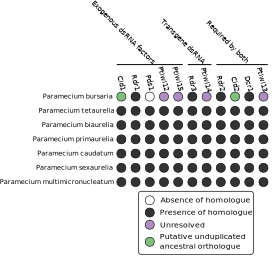
\includegraphics[width=\textwidth]{RNAi_factors_summary_figure.pdf}
    \caption[Summary of RNAi Factors Presence]{Summary of the discovery
    of RNAi figures in \textit{P. bursaria}}
    \label{fig:rnai_summary}
\end{figure}

Two proteins essential for the function of the exogenous dsRNA induced
RNAi pathway in \textit{P. tetaurelia}, Psd1 and Rdr1, were not found in the partial genome and transcriptome 
of \textit{P. bursaria} CCAP 1660/12 or the transcriptome of \textit{P. bursaria} YADG1N.
This suggests that this pathway may not be active/present in \textit{P. bursaria}.
Either, 


However, assuming the likely pre-duplication orthologue of Cid2 and the necessary 
unresolved Ptiwi's are functional
in the transgene dsRNA pathway of \textit{P. bursaria}
then this pathway is theoretically active.  Unfortunately, methodological
difficulties in microinjection have thus far failed to generate RNAi-induced
phenotypes.
